\section{Details of Numerical Models for DEF Simulation}

\subsection{Introduction}

The exactly same model is used for DEF simulation in order to cross compare the cracking patterns and mechanical properties changes under ASR and DEF expansion.

\subsection{Geometry of Numerical Models}

The geometry of the models is exactly the same as models using in ASR simulation, which is in dimension of 100 x 100 x 100mm.

All materials properties are set to be exactly the same.

\subsection{Coarse Aggregate of Numerical Models}

To analysis the behavior of concrete with different coarse aggregate volume ratio, 15\% coarse aggregate model(Fig.X) and 30\% coarse aggregate model(Fig.X) are built for simulation.

\subsection{DEF Intensified Expansion Area of Numerical Models}

Since DEF is closely related to higher curing temperature, here we choose to intensified the expansion in center part of model.

Here we chooses 3 cases in different expansion intensified area. The \textbf{table \ref{table:DEF_X}} is a list of cases simulated.

\begin{table}[ht!]
\centering
\begin{tabular}{||c c c||}
 \hline
 Case &  Expansion Intensified Depth[mm] &  Expansion Intensified Area[\%] \\ [0.5ex]
 \hline\hline
 1 & 0 & 100 \\
 2 & 12.5 & 56.25 \\
 3 & 25 & 25 \\ [0.5ex]
 \hline
\end{tabular}
\caption{DEF Intensified Expansion Area}
\label{table:DEF_X}
\end{table}

\begin{figure}[ht]
\centering
    %*******
    \begin{subfigure}{.33\textwidth}
      \centering
      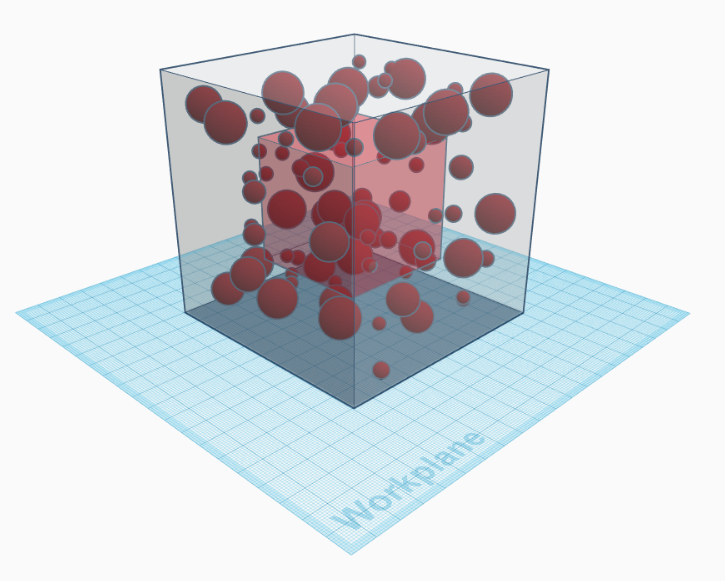
\includegraphics[width=.8\linewidth]{Files/DEF_X/X0_3d.png}
      \caption{Intensified  \\ 50x50x50mm Case}
    \end{subfigure}%
    %*******
    \begin{subfigure}{.33\textwidth}
      \centering
      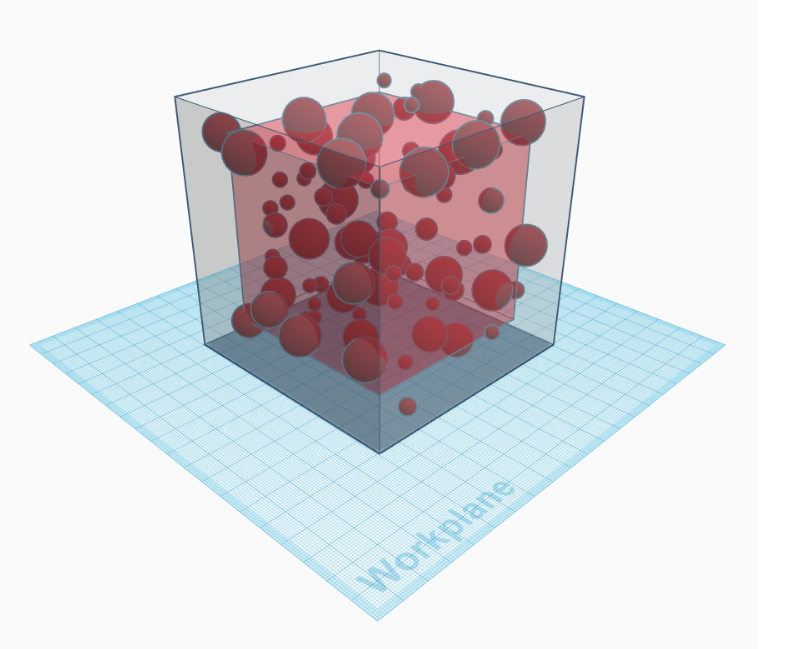
\includegraphics[width=.8\linewidth]{Files/DEF_X/X-5_3d.png}
      \caption{Intensified  \\ 75x75x75mm Case}
    \end{subfigure}%
    %*******
    \begin{subfigure}{.33\textwidth}
      \centering
      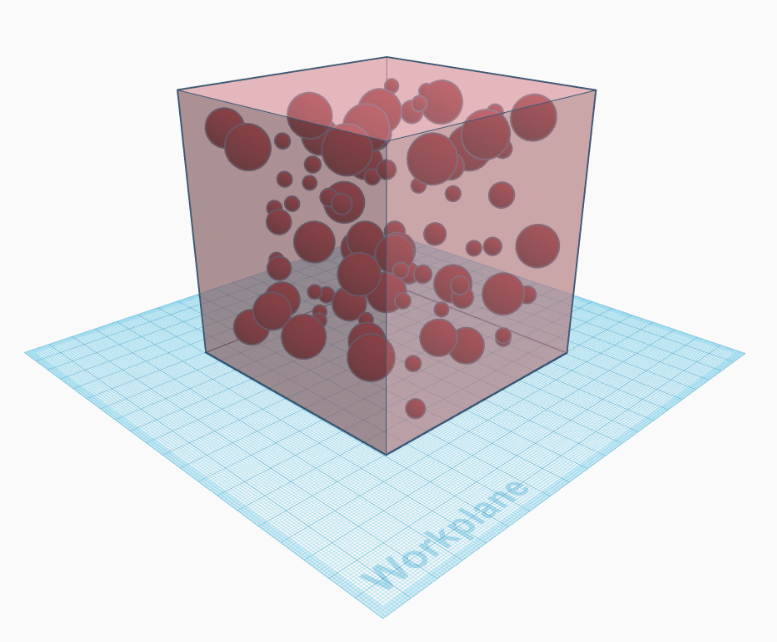
\includegraphics[width=.8\linewidth]{Files/DEF_X/X-1_3d.png}
      \caption{Intensified  \\ 100x100x100mm Case}
    \end{subfigure}
    %*******
    %*******
    \begin{subfigure}{.33\textwidth}
      \centering
      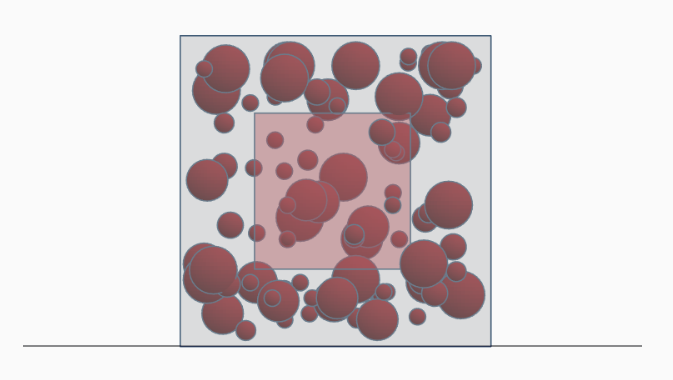
\includegraphics[width=.8\linewidth]{Files/DEF_X/X0_3ds.png}
      \caption{Intensified  \\ 50x50x50mm Case\\ Cross Section}
    \end{subfigure}%
    %*******
    \begin{subfigure}{.33\textwidth}
      \centering
      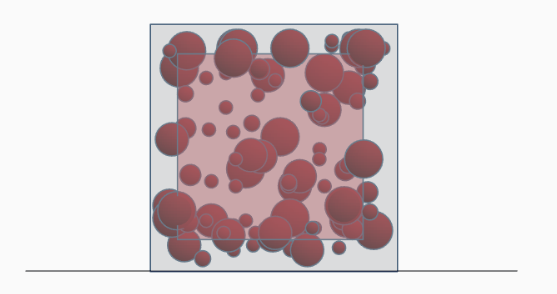
\includegraphics[width=.8\linewidth]{Files/DEF_X/X-5_3ds.png}
      \caption{Intensified \\  75x75x75mm Case \\ Cross Section}
    \end{subfigure}%
    %*******
    \begin{subfigure}{.33\textwidth}
      \centering
      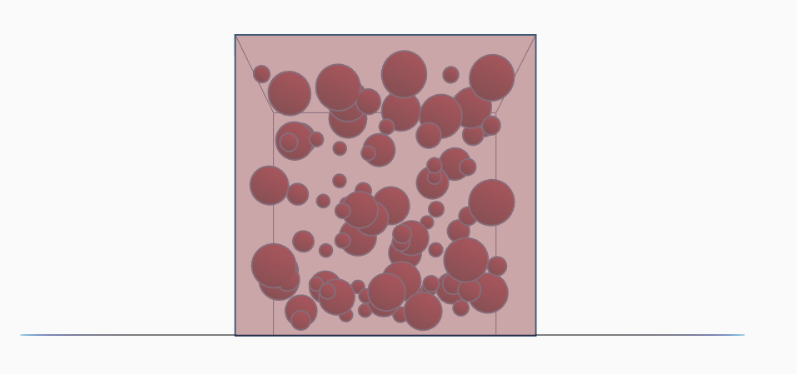
\includegraphics[width=.9\linewidth]{Files/DEF_X/X-1_3ds.png}
      \caption{Intensified  \\ 100x100x100mm Case\\ Cross Section}
    \end{subfigure}
    %*******
  \caption{DEF intensified part range}
  \label{fig:DEF_X}
\end{figure}

\subsection{Boundary Conditions}

\subsubsection{Boundary Condition During DEF Expansion}

Same as in ASR expansion, during DEF expansion, no confinements are added to the boundary elements. Models expanse freely in all directions.

\subsubsection{Boundary Conditions During Uni-axial Loading Test}

Same as in ASR expansion, Uni-axial Loading Test is applied with both fixed and free boundary conditions.

\begin{figure}[h!]
  \centering
  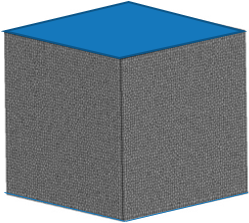
\includegraphics{Files/Background/LOAD.png}
  \caption{Top and Bottom Boundary in Loading}
  \label{boundary}
\end{figure}

In the case of fixed boundary condition, displacement in all directions are assumed as 0 at the bottom. Displacement in horizontal directions are all assumed as 0 at the top, and displacement in vertical direction is increased by 0.02mm downward at each loading step.

In the case of free boundary condition, all boundary elements able to move freely in horizontal direction except 2 center elements in top and bottom are fixed in horizontal direction, to prevent the sliding of whole model during loading. Same as fixed boundary condition cases, displacement in vertical direction is increased by 0.02mm downward at each loading step for top boundary elements.

Loading is applied until the maximum compressive strength is reached.
